\chapter*{Conclusioni}
	\addcontentsline{toc}{chapter}{Conclusioni}
	\markboth{\textsc{\uppercase{Conclusioni}}}{\textsc{\uppercase{Conclusioni}}}
	
	\addtocontents{lof}{~\hfill\par}
	\renewcommand\thefigure{C.\arabic{figure}}
	\setcounter{figure}{0}

	Chiudiamo questo elaborato con alcune conclusioni generali sul progetto, le modalità e gli strumenti utilizzati, facendo anche alcune considerazioni personali. Esporremo brevemente anche un altro progetto universitario nel quale abbiamo utilizzato e sfruttato le conoscenze apprese durante il corso di Data Warehousing.\\
	\\
	Il progetto che abbiamo seguito per la compilazione di questo elaborato è stato molto interessante, sia per quello che ci ha insegnato (come teoria, tecniche e strumenti) che per le possibilità che ci ha aperto nell'ambito dell'analisi \textit{OLAP} e del Data Warehousing in generale. La cosa interessante è che in questo progetto abbiamo potuto studiare ed applicare le tecniche di DW non ad un problema ``giocattolo'' (come spesso accade in ambito scolastico/universitario) ma ad un problema reale e non banale, come l'analisi del bilancio del Comune di Firenze. Ovviamente non ci siamo dilungati troppo sulle conclusioni delle singole analisi, in quanto non fa parte delle nostre competenze, ma abbiamo invece mostrato come sia semplice, tramite l'utilizzo di queste tecniche e strumenti, mettere a disposizione anche ad un esperto del settore tutti i dati e le analisi ricavate.\\
	Oltre a queste motivazioni, questo progetto ci ha anche ``insegnato'' ad utilizzare il sistema Pentaho che, come indicato più avanti, abbiamo già saputo sfruttare in altri ambiti.

	\section*{Alcune considerazioni}
		\addcontentsline{toc}{section}{Alcune considerazioni}
		\markright{\textsc{\uppercase{Alcune considerazioni}}}

		Alcune considerazioni vanno fatte riguardo i \textit{dataset utilizzati} ed il sito degli OpenData del Comune di Firenze\footnote{\url{http://opendata.comune.fi.it/}}: senza ombra di dubbio il Comune di Firenze ha fatto grandi passi, negli ultimi anni, in ambiente informatico e la scelta degli OpenData è senz'altro la direzione giusta da seguire. Tuttavia il Comune è ancora lontano dalla ``perfezione'': la maggior parte dei \textit{dataset} pubblicati sul sito sono parziali, incompleti, inconsistenti e molto probabilmente anche pieni di errori. Inoltre molti \textit{dataset} presenti hanno un livello aggregazione talmente elevato da impedire qualsiasi analisi su di essi che non sia priva di significato.\\
		\\
		Per quanto riguarda il nostro progetto non è stato facile individuare all'interno del sito questi due \textit{dataset} che facessero al caso nostro, in quanto tutti gli altri impedivano, in un modo o nell'altro, delle analisi ragionevoli.\\
		Inoltre potremmo aggiungere che, nonostante i due \textit{dataset} dei bilanci 2012/2013 siano piuttosto ricchi e ben strutturati, si sarebbero potute aggiungere tante informazioni aggiuntive, come ad esempio se una o più commissioni fanno parte di un particolare progetto del Comune oppure il tipo di ogni commissione (ad esempio lavori di ampliamento, di ristrutturazione, di installazione di nuovi servizi, ecc\dots), dando la possibilità di effettuare molte più analisi su di essi.\\
		\\
		Siamo quindi rimasti contenti dal progetto OpenData del Comune di Firenze, con la speranza che il lavoro in questo senso sia solo agli inizi e che negli anni avvenire si registri un incremento nell'affluenza di dati e magari un maggior controllo e lavoro di ripulitura su quest'ultimi.

	\section*{Altri progetti}
		\addcontentsline{toc}{section}{Altri progetti}
		\markright{\textsc{\uppercase{Altri progetti}}}
	
		In quest'ultima sezione, riportiamo alcuni cenni ad un altro nostro utilizzo di Pentaho, nell'ambito di un altro progetto universitario. Il progetto in questione, relativo al corso di \textit{AQS} (\textit{Analisi Quantitativa dei Sistemi}, Corso di Laurea Magistrale in Informatica) aveva come obiettivo la caratterizzazione del comportamento temporale del tool \textit{Snort}, un sistema di \textit{Network Intrusion Detection} (\textit{NIDS}).\\
		La prima parte del progetto si compone essenzialmente di un'analisi sperimentale, la quale produce una grossa mole di dati che, nella seconda parte del progetto, sarà necessario interpretare e analizzare per rispondere a quanto chiesto.\\
		\\
		Per integrare e manipolare i dati raccolti abbiamo scelto di utilizzare Pentaho al fine di generare successivamente un sistema \textit{OLAP} su cui effettuare tutte le analisi necessarie.\\
		Senza entrare nel merito di quelli che sono i contenuti ed i significati dei file \texttt{.csv} generati in fase sperimentale, riportiamo qui la trasformazione \textit{Kettle} eseguita su di essi. Utilizzando il tool \textit{Kettle} è possibile infatti integrare e manipolare i file \texttt{.csv} generati in fase sperimentale, così da renderli in una forma più consona alla memorizzazione all'interno di un database: sarà possibile, ad esempio, modificare alcuni campi o aggiungerne di nuovi come campi calcolati.\\
		Vediamo qui di seguito la trasformazione (per comodità divisa in quattro immagini) che permetterà di integrare tra loro i dati relativi ai vari esperimenti eseguiti:
		
		\begin{figure}[h!]
			\centering
			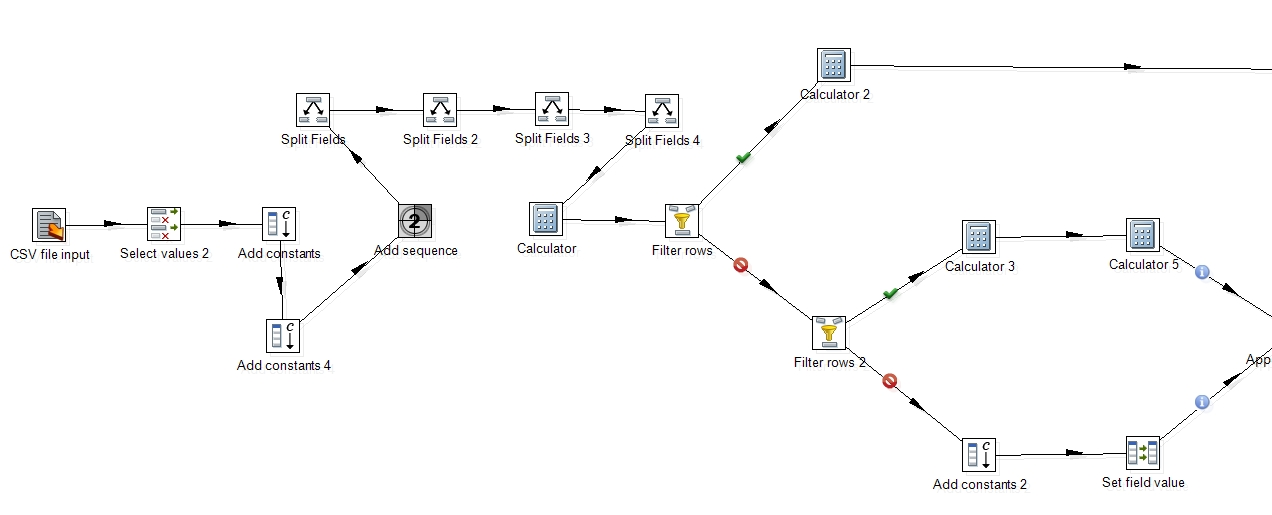
\includegraphics[scale=0.4]{kettle1.jpg}
			\caption{AQS: trasformazione \textit{Kettle}, prima parte.}
			\label{fig:kettle1}
		\end{figure}
	
	    \begin{figure}[h!]
			\centering
			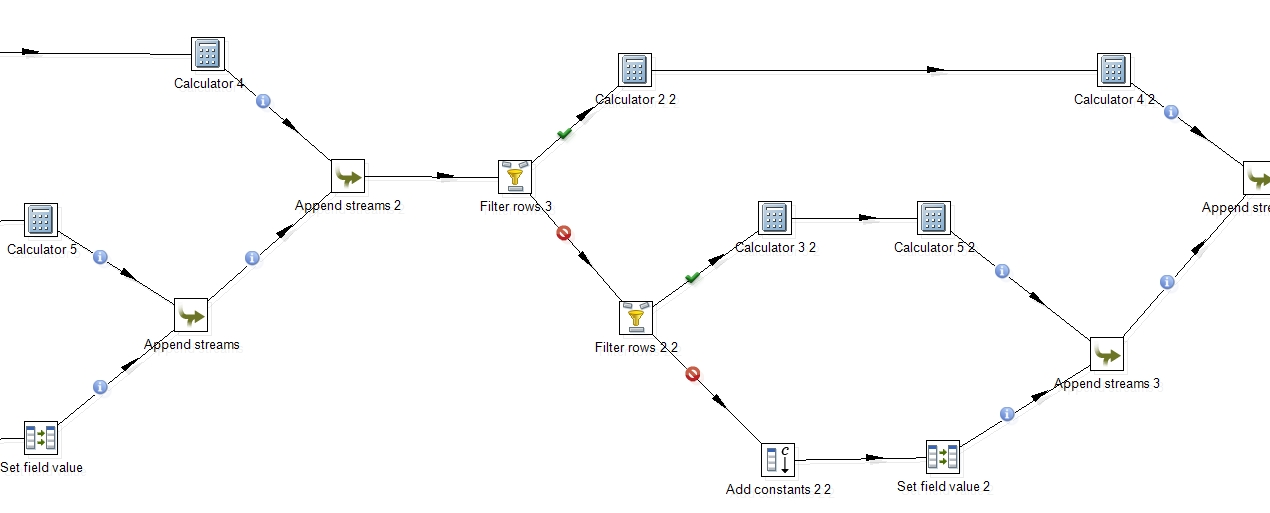
\includegraphics[scale=0.4]{kettle2.jpg}
			\caption{AQS: trasformazione \textit{Kettle}, seconda parte.}
			\label{fig:kettle2}
		\end{figure}
	
	    \begin{figure}[h!]
			\centering
			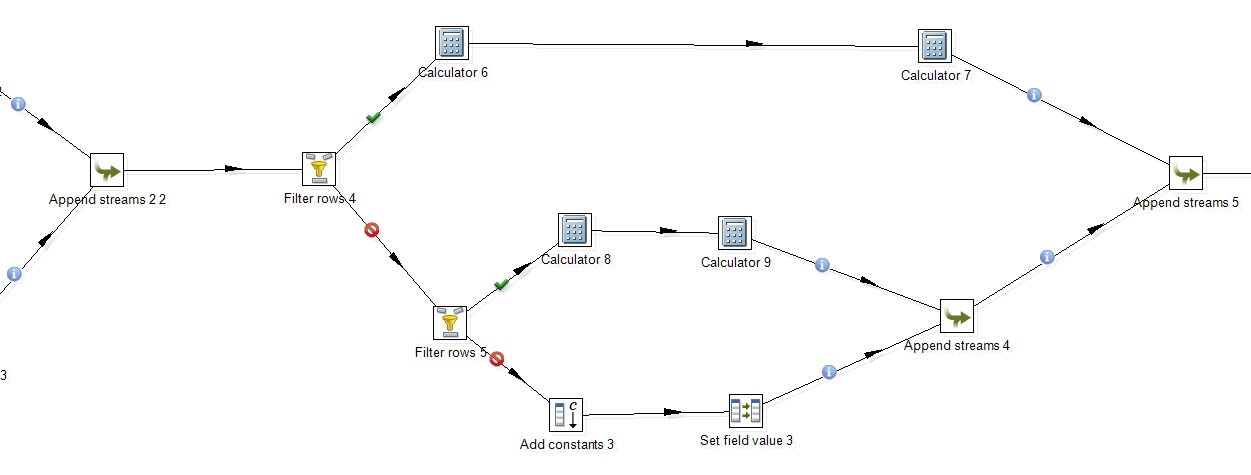
\includegraphics[scale=0.4]{kettle3.jpg}
			\caption{AQS: trasformazione \textit{Kettle}, terza parte.}
			\label{fig:kettle3}
		\end{figure}
	
	    \begin{figure}[h!]
			\centering
			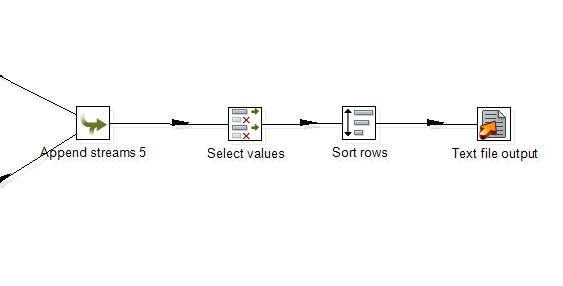
\includegraphics[scale=0.4]{kettle4.jpg}
			\caption{AQS: trasformazione \textit{Kettle}, quarta parte.}
			\label{fig:kettle4}
		\end{figure}
	
		Il file generato da \textit{Kettle} (file di log \texttt{logCompleto.csv}), ancora in formato \texttt{.csv}, consiste nell'elenco di tutti i pacchetti loggati a cui erano associate tutte le informazioni registrate durante gli esperimenti.\\
		A partire dal \texttt{.csv} generato da \textit{Kettle}, utilizzando il tool \textit{Mondrian} è stato possibile definire uno \textit{star-schema}, con la struttura indicata in Figura \ref{fig:star}.
		
		\begin{figure}[h!]
			\centering
			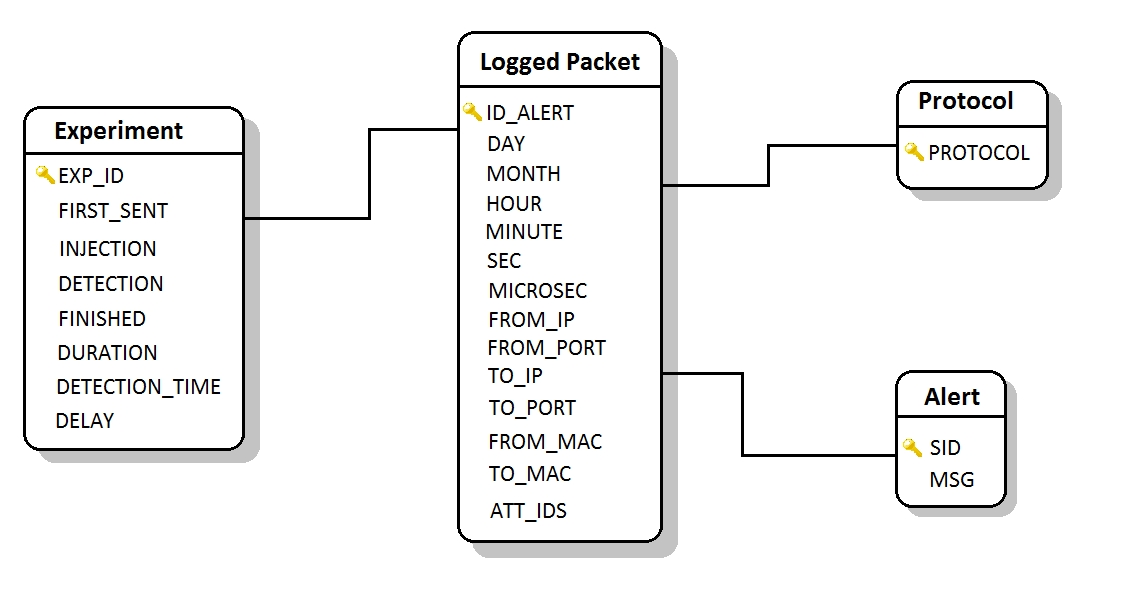
\includegraphics[scale=0.45]{star-schema.jpg}
			\caption{\textit{Schema a stella} costruito sul file di log finale.}
			\label{fig:star}
		\end{figure}
		
		Questa struttura ci ha permesso di modellare il fatto \textit{Logged Packet}. L'analisi, infatti, è volta ad analizzare come Snort reagisce e varia le proprie prestazioni al variare sia di tool di \textit{fault injection} che, pur rimanendo all'interno dello stesso tool, delle opzioni attive.\\
		A partire da questo schema a stella, eseguendo sostanzialmente gli stessi procedimenti descritti nelle sezioni precedenti abbiamo eseguito tutte le analisi del caso, ottenendo grafici e tutte le considerazioni necessarie per una completa caratterizzazione del comportamento di Snort. Alcuni esempi a riguardo sono riportati nelle Figure \ref{fig:duration_protocol} e \ref{fig:tempi_nmap_T}.
		
		\begin{figure}[h!]
			\centering
			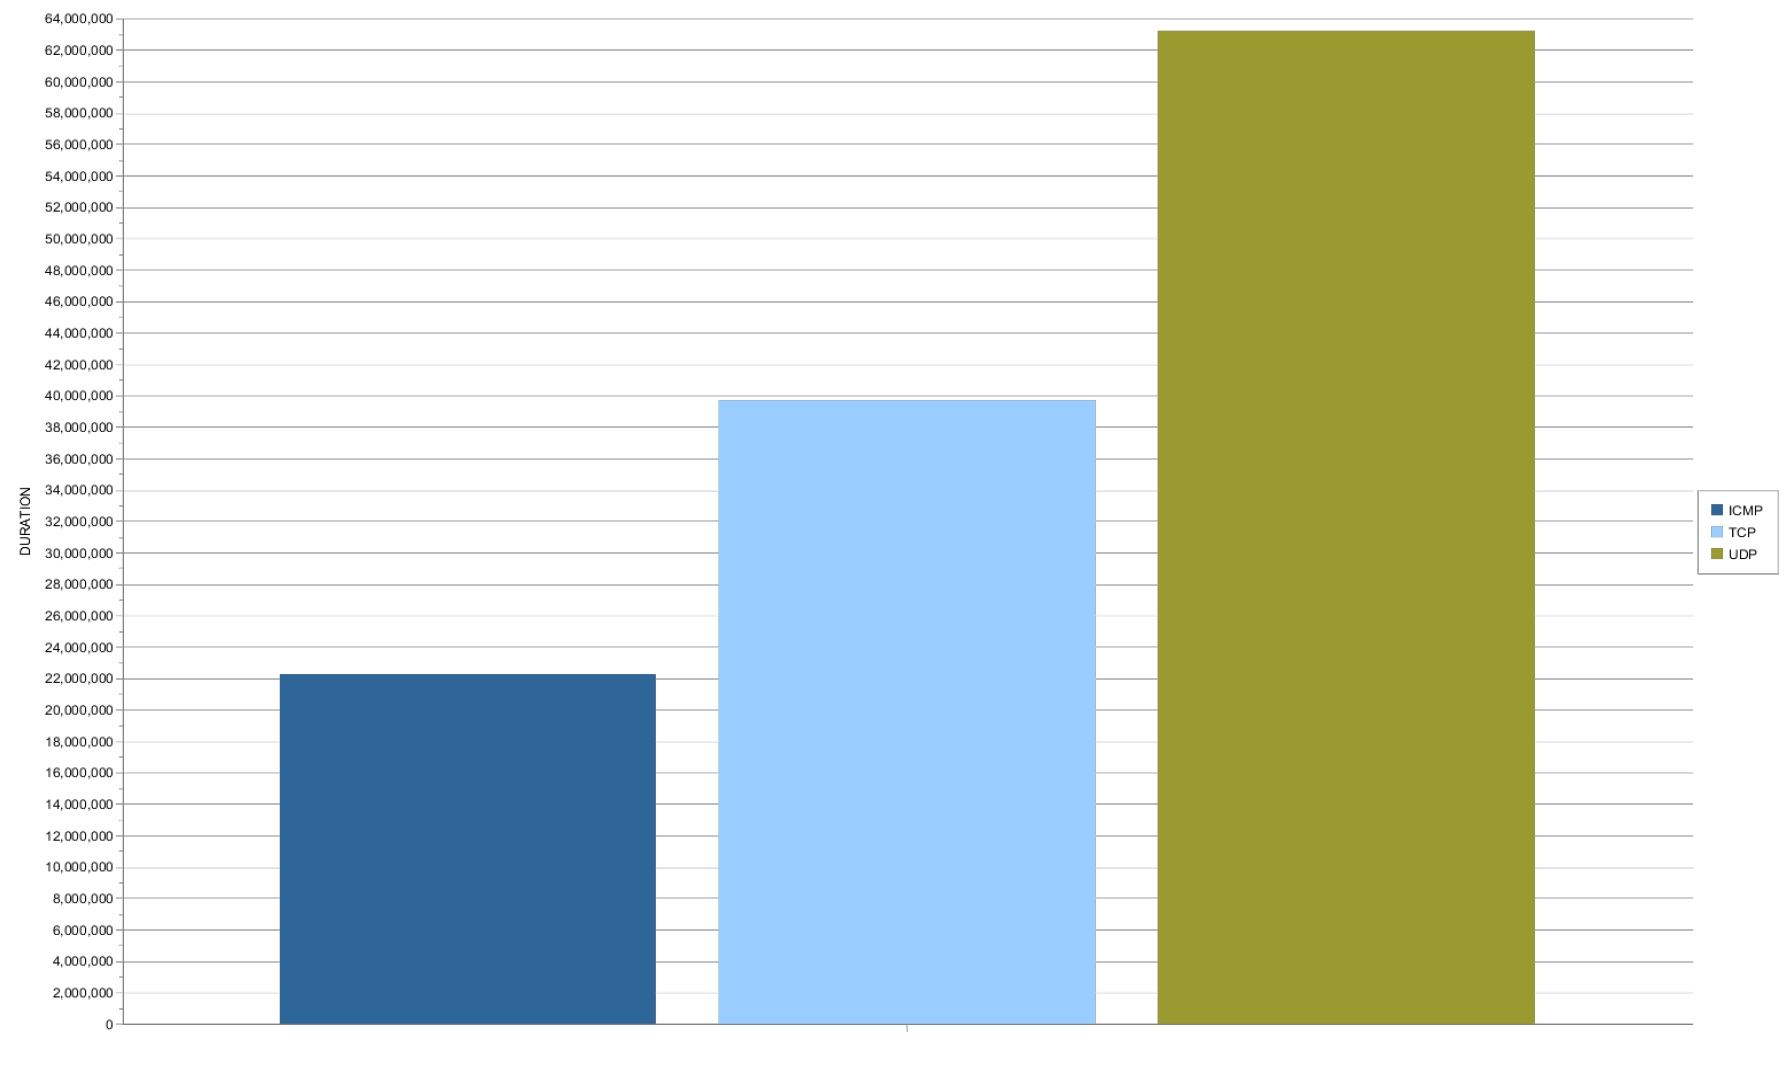
\includegraphics[scale=0.3]{duration_protocol.jpg}
			\caption{Durata media degli attacchi per protocollo.}
			\label{fig:duration_protocol}
		\end{figure}
		
		\begin{figure}[h!]
			\centering
			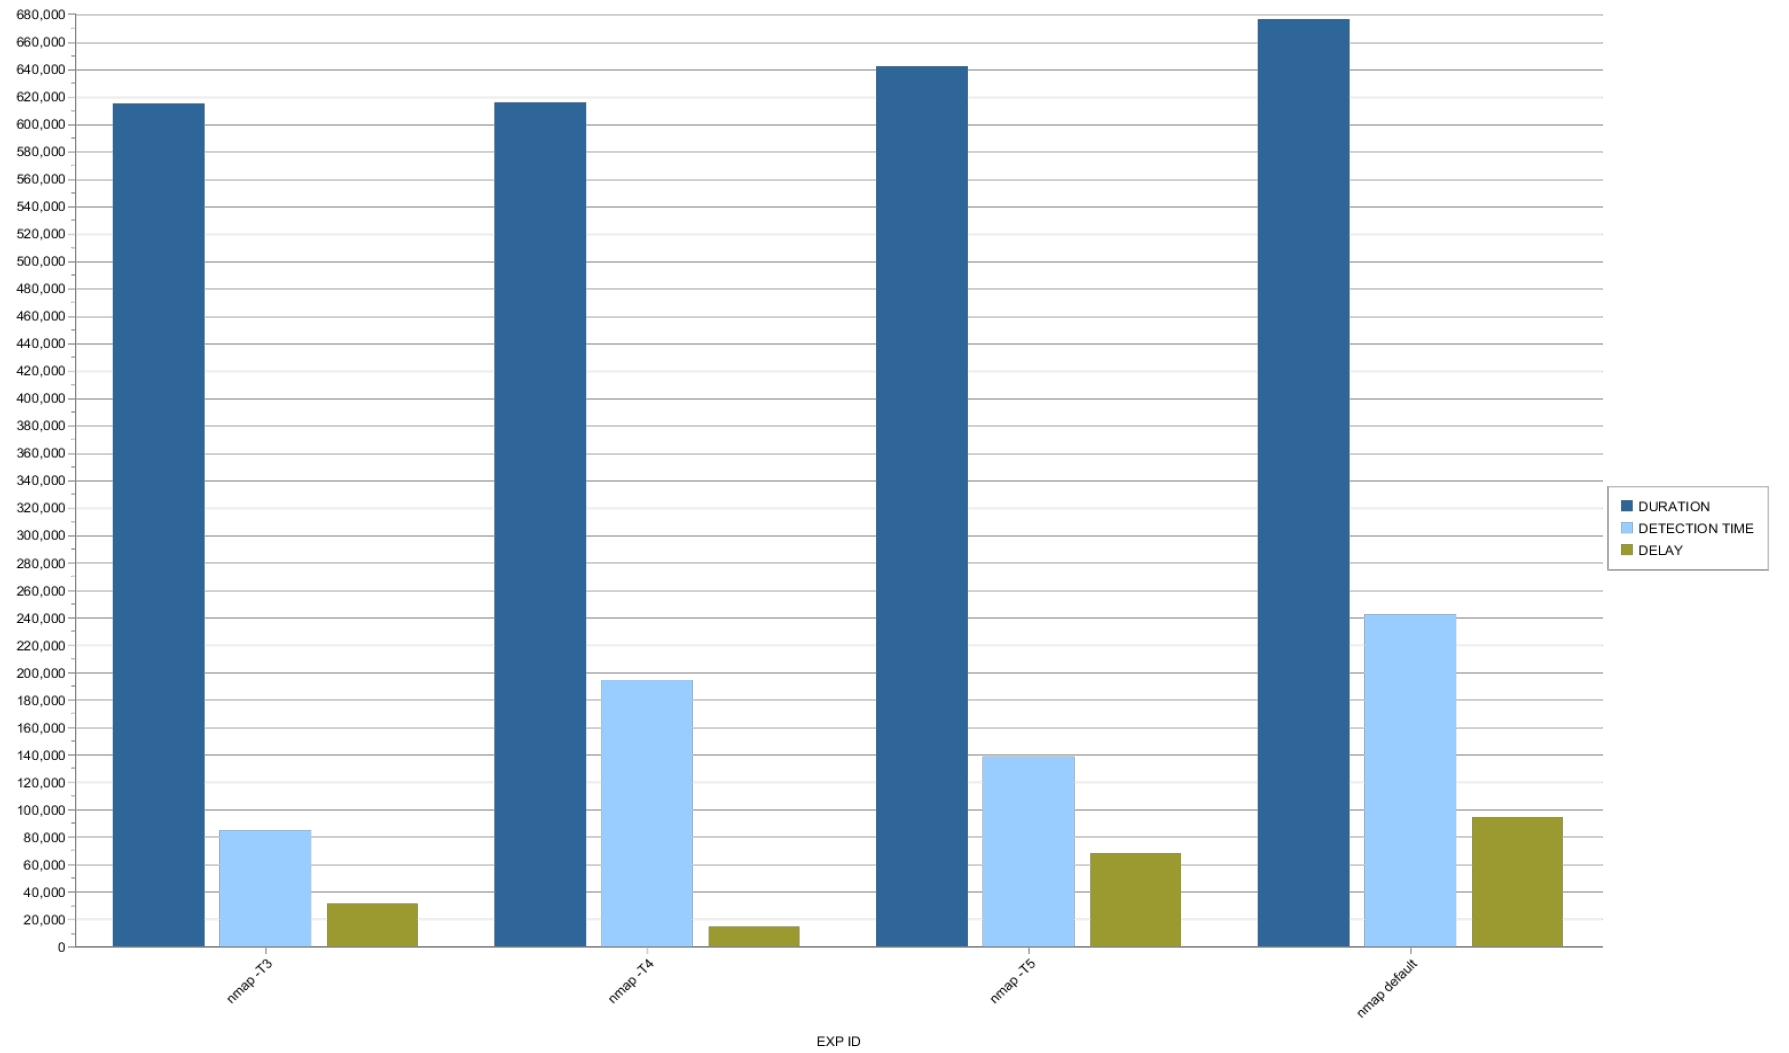
\includegraphics[scale=0.3]{tempi_nmap_T.jpg}
			\caption{Tempistiche dell'attacco \textit{nmap} con opzione \texttt{-T}.}
			\label{fig:tempi_nmap_T}
		\end{figure}